% !TeX spellcheck = de_DE
\documentclass[12pt,parskip=full]{scrartcl}
 
\usepackage[utf8]{inputenc}
\usepackage[T1]{fontenc}
\usepackage{lmodern}
\usepackage[ngerman]{babel}
\usepackage{color}
\usepackage{amsmath,amssymb,amstext,mathtools,amsthm}
\usepackage{subcaption}
\usepackage{float}
\usepackage{stmaryrd}
\usepackage[hidelinks]{hyperref}
\hypersetup{bookmarksnumbered}

\usepackage{tikz}
\usetikzlibrary{positioning}

\usepackage{enumitem}
\setenumerate{label=\arabic*)}

\newcommand{\setN}{\mathbb{N}}
\newcommand{\setZ}{\mathbb{Z}}
\newcommand{\setQ}{\mathbb{Q}}
\newcommand{\setR}{\mathbb{R}}
\newcommand{\setC}{\mathbb{C}}
\newcommand{\setH}{\mathbb{H}}
\newcommand{\setk}{\Bbbk}
\newcommand{\ldot}{\,.\,}
\newcommand{\Forall}{~\forall}
\newcommand{\Exists}{~\exists}

\newcommand{\abs}[1]{{\left| #1 \right|}}
\newcommand{\dabs}[1]{{\left\lVert #1 \right\rVert}}
\newcommand{\heading}{\underline}
 
\DeclareMathOperator{\Kons}{Kons}
\DeclareMathOperator{\charac}{char}
 
\theoremstyle{definition}
\newtheorem{theorem}{Satz}[section]
\newtheorem{corollary}[theorem]{Folgerung}
\newtheorem{proposition}[theorem]{Proposition}
\newtheorem{lemma}[theorem]{Lemma}
\newtheorem{definition}[theorem]{Definition}
\newtheorem{example}[theorem]{Beispiel}
\newtheorem*{axiom}{Axiom}

 
\theoremstyle{remark}
\newtheorem*{remark}{Bemerkung}
 
\hfuzz=5pt 
 
\title{Skript Algebra}
\author{Lukas Metzger}
\date{\today}
 
\begin{document}
	\maketitle
	
	\setcounter{section}{-1}
	\section{Konstruktion mit Zirkel und Lineal}
	
	\begin{example}[Konstruktion des regelmäßigen 5-Ecks]
		Anleitung zur Konstruktion
		\begin{center}
			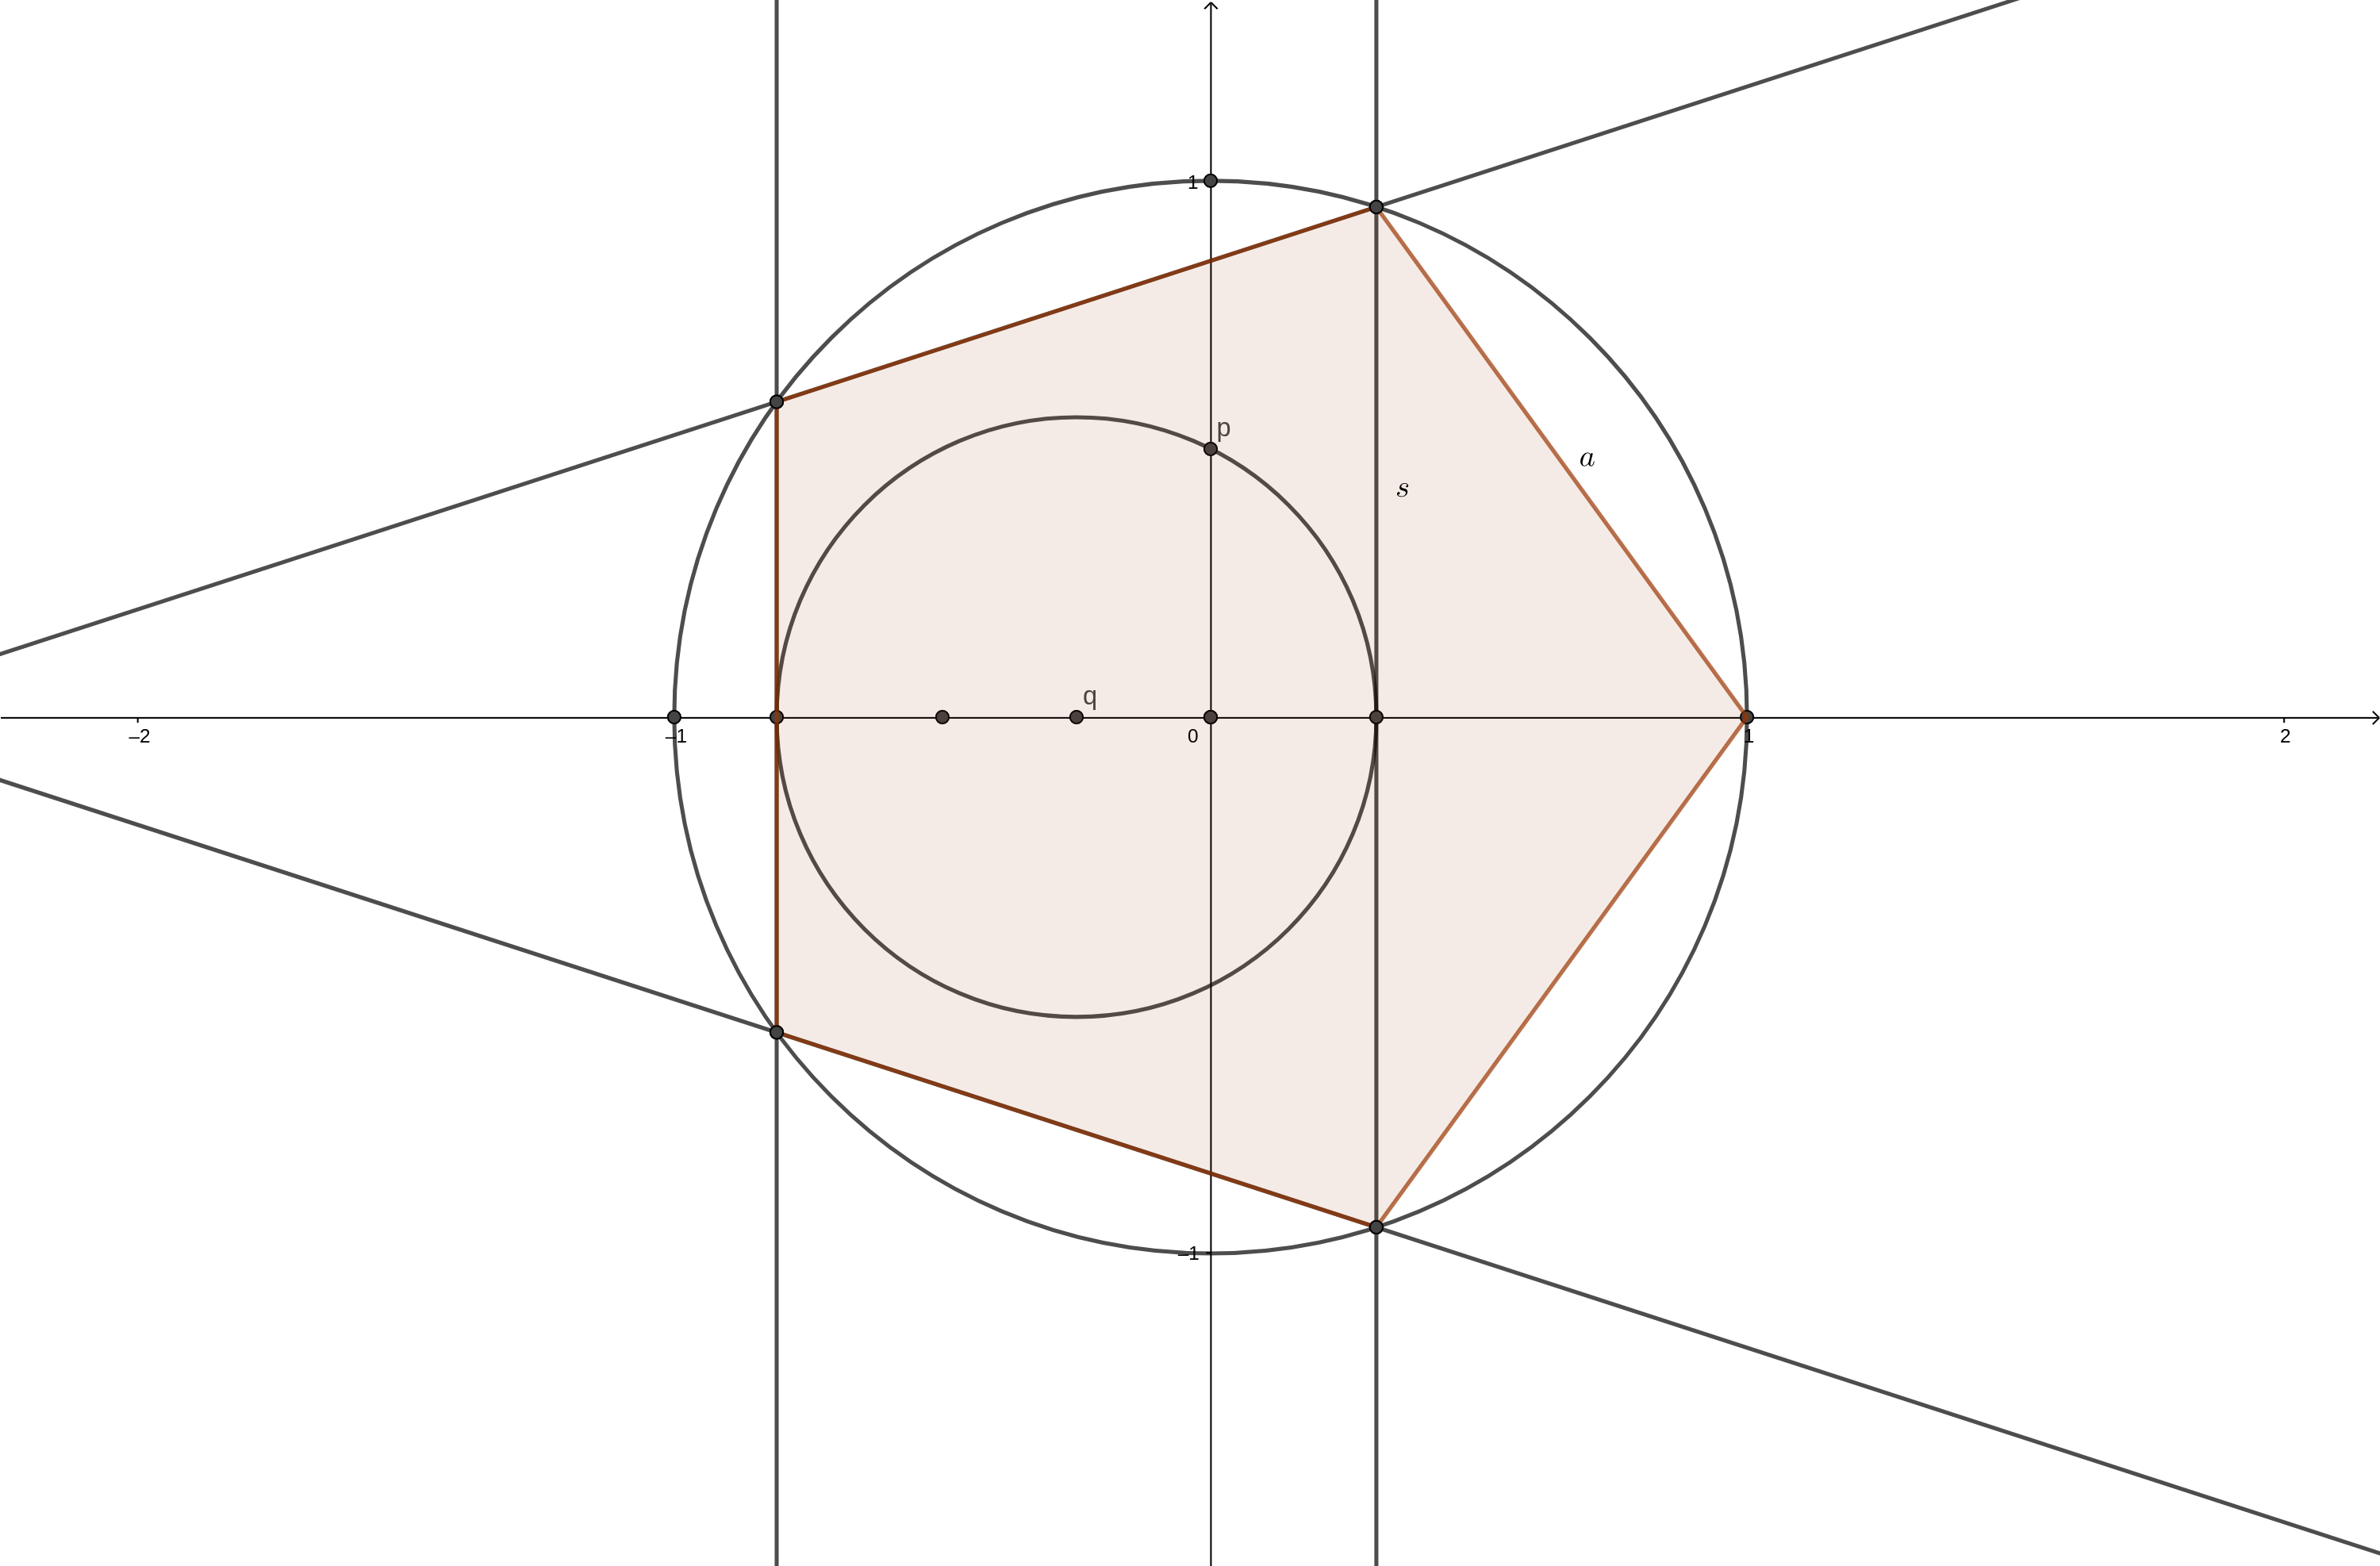
\includegraphics[width=0.8\linewidth]{bilder/bild1.png}
		\end{center}
	\end{example}

	\heading{Erste Frage:} Gegeben $n \in \setN$, kann ich das regelmäßige $n$-Eck konstruieren?
	
	\heading{Beispielproblem:} Betrachte Das $5$-Eck, sei $a$ die Kantenkänge und $s$ die Sekantenlänge.
	
	Dann ist $\frac{s}{a} \notin \setQ$.
	
	\begin{proof}
		Angenommen $\frac{s}{a}$ wäre in $\setQ$. Dann schreibe $\frac{s}{a} = \frac{p}{q}$ mit $p,q \in \setN$. Dann gibt es also eine Länge $d \in \setR$, so dass $s$ und $a$ beides ganzzahlige Vielfache von $d$ sind. $\exists n,m \in \setN$  $a = n \cdot d, s= m \cdot d$.
		
		Betrachte/Erweitere die Konstruktion des $5$-Ecks und erhalte kleines (blaues) $5$-Eck wie gezeichnet mit Sekantenlänge $s' = a$ und Kantenlänge $a' = s - a$.
		
		\begin{center}
			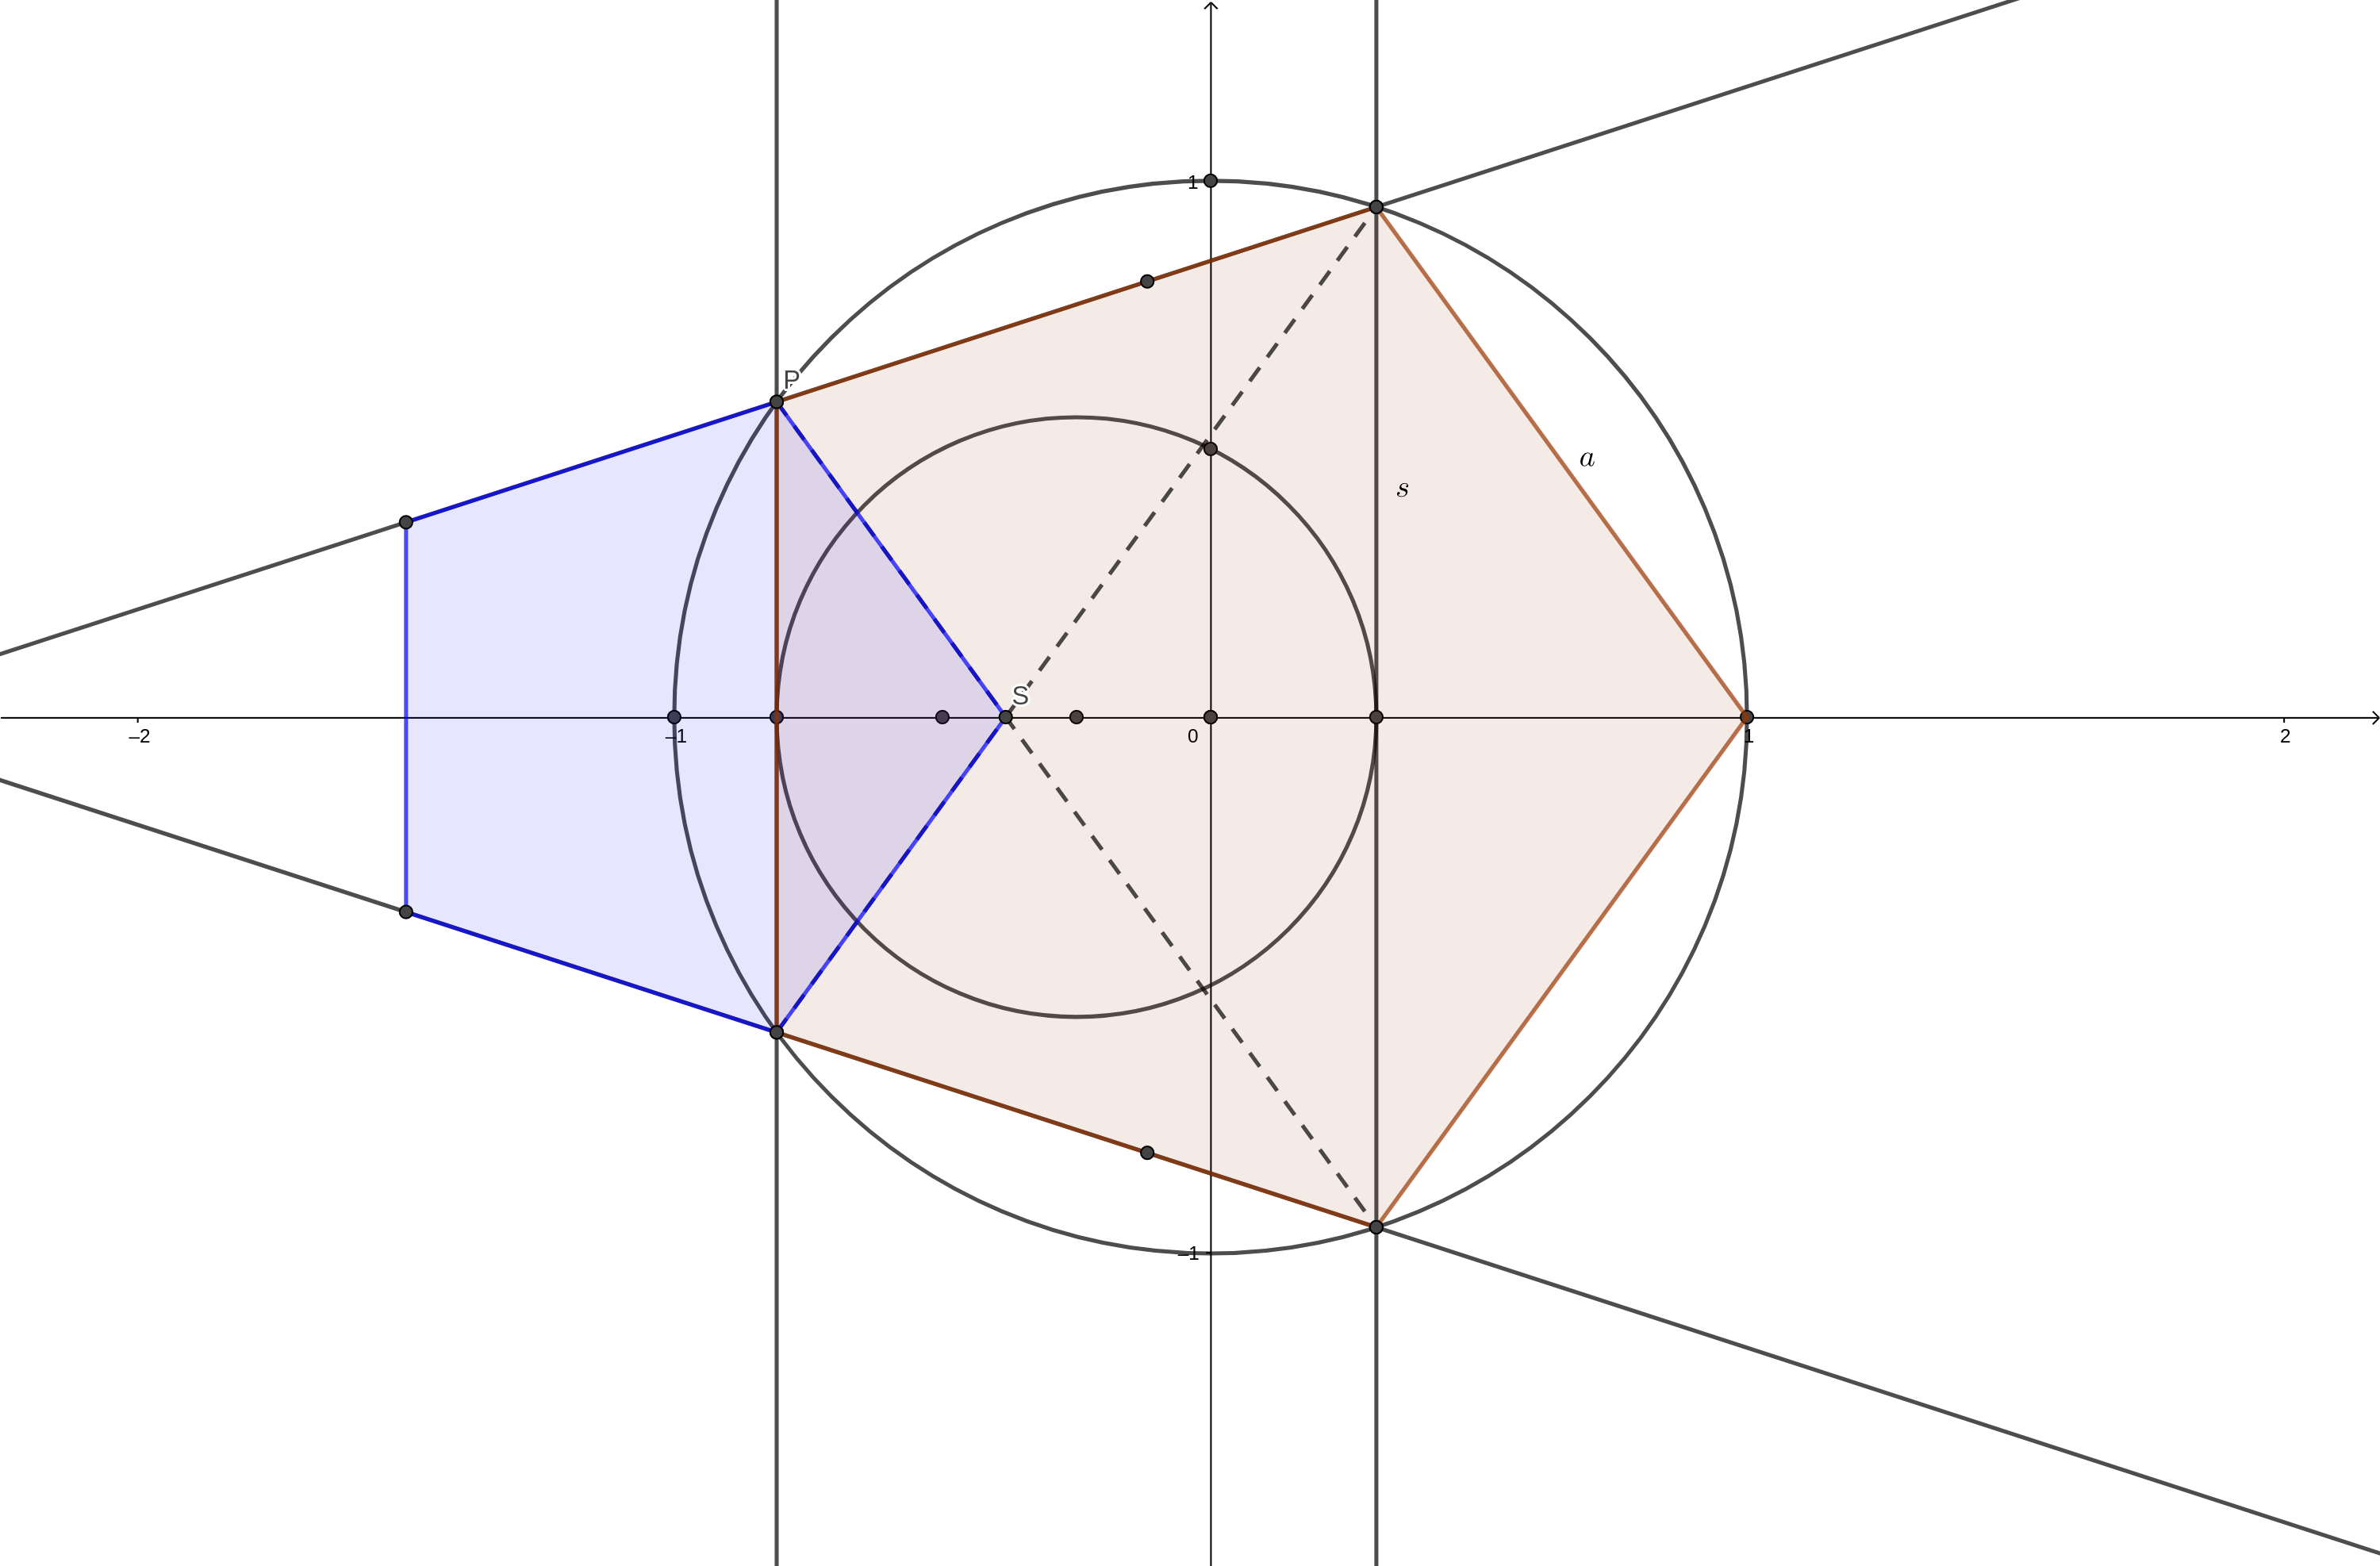
\includegraphics[width=0.8\linewidth]{bilder/bild2.png}
		\end{center}
	
		Dann sind aber sowohl $a'$ als auch $s'$ wieder Vielfache von $d$. Das Verfahren kann ich wiederholen und erhalte immer kleinere $5$-Ecke, deren Größe nach $0$ konvergiert, wo Kanten- und Sekantenlänge ganzzahlige Vielfache von $d$ sind. $\lightning$
	\end{proof}

	\heading{Weitere Konstruktionsprobleme:}
	\begin{itemize}
		\item $3$-Teilung des Winkels
		\item Verdoppelung des Würfels (d.h. Verdoppelung des Volumens)
		\item Quadratur des Kreises (Gegeben ein Kreis, konstruiere Quadrat mit demselben Flächeninhalt)
	\end{itemize}

	\heading{Wiederholung:} Was kann ich mit Zirkel und Lineal eigentlich machen?
	
	Antwort: $3$ Konstruktionen
	\begin{enumerate}
		\item Gegeben Punkte $a_1, a_2, b_1, b_2$ der Ebene, betrachte die Geraden $\overline{a_1 a_2}$ und $b_1 b_2$ und erhalte Schnittpunkt $\overline{a_1 a_2} \cap \overline{b_1 b_2}$.
		\item Gegeben Punkte $a_1, a_2, b_1, b_2, b_3$ der Ebene betrachte Kreis $K(b_1, \dabs{b_2 - b_3})$ um $b_1$ mit Radius $\dabs{b_2 - b_3}$ und erhalte die Schnittpunkte $\overline{a_1 a_2} \cap K(b_1, \dabs{b_2 - b_3})$
		\item Gegeben Punkte $a_1, a_2, a_3, b_1, b_2, b_3$, erhalte Schnittpunkte $K(a_1, \dabs{a_2 - a_3}) \cap K(b_1, \dabs{b_2 - b_3})$
	\end{enumerate}

	\begin{definition}
		Sei $M \subset \setR^2$ eine Menge, $p \in \setR^2$ ein Punkt.
		
		Sage: $p$ ist aus $M$ mit Zirkel und Lineal konstruierbar, falls es Kette von Mengen gibt
		\begin{equation*}
			M = M_1 \subseteq M_1 \subseteq \dots \subseteq M_n \ni p
		\end{equation*}
		Wobei $\forall i$ die Menge $M_i$ entsteht aus $M_{i-1}$ durch Hinzunahme der Punkte die durch einen Konstruktionsschritt entstehen.
	\end{definition}

	\heading{Historie:} Einen Durchbruch bei der Lösung dieser Probleme gab es erst, als man begann, die Punkte des $\setR^2$ mit komplexen Zahlen zu identifizieren.
	
	\begin{remark}
		Frage nach der Konstruierbarkeit macht nur Sinn, wenn $M$ mindestens $2$ Punkte enthält $\leadsto$ Häufig $M = \{0,1\} \subset \setC$.
	\end{remark}

	\heading{In dieser Sprache}
	\begin{itemize}
		\item Konstruktionsproblem: $n$-Eck ist äquivalent zu, kann ich die $n$-ten Einheitswurzeln $e^{\frac{i 2 \pi}{n}}$ aus $M = \{ 0,1 \}$ konstruieren?
		Ist $e^{\frac{2\pi i}{n}} \in \Kons(\{0,1\})$?
		\item Verdopplung des Würfels $\Leftrightarrow$ Ist $\sqrt[3]{2} \in \Kons(\{0,1\})$
		\item Quadratur des Kreises $\Leftrightarrow$ Ist $\sqrt{\pi} \in \Kons(\{0,1\})$
		\item $3$-teilung des Winkels $\Leftrightarrow$ Ist für gegebenes $\varphi \in (0,2\pi)$ $e^{\frac{i \varphi}{3}} \in \Kons(\{ 0, 1, e^{i \varphi} \})$
	\end{itemize}

	\heading{Zentrale Beobachtung}
	
	Sei $M \subset \setC$ eine Menge die $0$ und $1$ enthält. Sei $\Kons(M)$ die Menge der aus $M$ konstruierbaren Punkte.
	
	Dann ist $\Kons(M) \subset \setC$ ein Unterkörper.
	
	\textit{Dazu zu prüfen:} Konstruierbarkeit von Summen, Differenzen, Produkten, Quotienten \dots.
	
	\heading{Zusammenfassung/zentrales Thema der Vorlesung}
	
	Körpererweiterung / wie können Körper ineinander enthalten sein?	
	
	\section{Körpererweiterungen}
	
	\subsection{Ultrakurzwiederholung zentraler Begriffe}
	
	\begin{definition}[Gruppe]
		Eine Gruppe ist eine Menge $G$ zusammen mit einer Abbildung $m: G \times G \to G$ so dass folgendes gilt:
		\begin{enumerate}
			\item Assoziativ: $\forall a,b,c \in G \, m(m(a,b), c) = m(a, m(b,c))$
			\item Neutrales Element: $\exists n \in G \forall a \in G: m(n,a) = m(a,n) = a$
			\item Inverse Elemente: $\forall a \in G \exists b \in G: ab = ba$ und dieses Produkt ist neutrales Element wie in $2)$
		\end{enumerate}
	\end{definition}

	\begin{lemma}[Elementare Eigenschaften von Gruppen]
		Für jede Gruppe gilt:
		\begin{itemize}
			\item Das neutrale Element ist eindeutig
			\item Inverse Elemente sind eindeutig
		\end{itemize}
	\end{lemma}

	\begin{definition}[Abelsche Gruppe]
		Nenne Gruppe $(G,m)$ Abelsch, falls $\forall a,b \in G: m(a,b) = m(b,a)$.
	\end{definition}

	\heading{Notation:} Statt $m$ schreibt man oft $+$ oder $\cdot$, wobei $+$ hauptsächlich für Abelsche Gruppen verwendet wird.
	
	\begin{example}
		Beispiele für Gruppen:
		\begin{itemize}
			\item Abelsche Gruppen: $(\setZ, +)$, $(\setZ / p\setZ, +)$, $(Vektorraum, +)$
			\item Nicht-Abelsche Gruppen: Sei $M$ eine Menge mit $>2$ Elementen. Die bijektiven Abbildungen $M \to M$ mit der Hintereinanderausführung ist eine nicht-Abelsche Gruppe.
			
			Sei $K$ ein Schiefkörper, z.B. $K = \setR, \setC, \setH$. Sei $K^* K \setminus \{0\}$. Dann ist $(K^*, \cdot)$ eine Gruppe.
			\item Nicht-Beispiel: $G = \setR^3$. Ich erhalte durch das Kreuzprodukt keine Gruppenkonstruktion.
		\end{itemize}
	\end{example}

	\begin{definition}[Ring]
		Ein Ring ist eine Menge $R$ mit $2$ Verknüpfungen $+$ und $\cdot$ so dass gilt:
		\begin{itemize}
			\item $(R,+)$ ist eine Abelsche Gruppe
			\item Distributivgesetz: $\forall a,b,c \in T (a+b) \cdot c = ac + bc$ und $a(b+c) = ab + ac$
			\item $(R \setminus 0, \cdot)$ ist fast Gruppe nämlich assoziativ und es existiert ein neutrales Element
		\end{itemize}
	\end{definition}

	\begin{example}
		Beispiele für Ringe:
		\begin{itemize}
			\item $\setR, \setZ / n\setZ$, Polynome, $\setZ$
			\item Funktionen auf $\setR / \setC$
			\item holomorphe/stetige/$C^\infty$/reell analytische lokal quadratintegrierbare Funktionen bilden ebenfalls einen Ring
		\end{itemize}
	\end{example}

	\begin{remark}
		Mit Ringen kann ich fast rechnen wie mit Zahlen, aber ACHTUNG
		\begin{itemize}
			\item Nicht jedes Element in $R \setminus 0$ hat ein multiplikatives Inverses
			\item Ich kann aus $a \cdot b = 0$ und $a \neq 0$ im Allgemeinen nicht folgern, dass $b = 0$
			\item Ich kann aus $ab = ac$ und $a \neq 0$ im allgemeinen nicht folgern, dass $b = c$ ist
		\end{itemize}
	\end{remark}

	\begin{definition}[Nullteiler]
		Sei $R$ ein Ring, $a \in R \setminus \{0\}$. Falls $b \neq 0$ existiert mit $a \cdot b = 0$, nenne ich $a$ einen Nullteiler.
		
		Ringe ohne Nullteiler heißen Nullteilerfrei oder Integritätsringe.
	\end{definition}

	\begin{definition}[Abelscher Ring]
		Ein Ring heißt abelsch, falls $\forall a,b \in R \; ab = ba$.
	\end{definition}

	\begin{remark}
		In der Literatur heißen unsere Ringe oft Ringe mit $1$.
	\end{remark}

	\begin{example}
		Beispiele zu Nullteilern
		\begin{itemize}
			\item $\setR, \setZ$ sind nullteilerfrei
			\item $\setZ / n \setZ$ ist nullteilerfrei $\Leftrightarrow$ $n$ ist Prim
			\item Polynome sind nullteilerfrei
			\item Stetige Funktionen sind nicht nullteilerfrei
		\end{itemize}
	\end{example}

	\begin{remark}
		Sei $R$ ein Ringe. Die Menge der Elemente, die ein multiplikatives Inverses haben, wir mit $R^*$ bezeichnet.
		
		\begin{itemize}
			\item $\setZ^* = \{ 1, -1 \}$
			\item $(\setZ / n \setZ)^* = \{ [x] \mid x \text{ ist teilerfremd zu } n \}$
			\item $(C^\infty(\setR))^* = \{ f: \setR \to \setR \mid \text{$f$ ist $C^\infty$ und hat keine Nullstelle} \}$
		\end{itemize}
	\end{remark}

	\begin{remark}
		Sei $R$ ein Ring, $x$ eine Variable. Dann bezeichne mit $R[x]$ die Polynome mit Koeffizienten in $R$ und Variable $x$.
		
		\begin{itemize}
			\item $1x + 2 \in \setZ[x]$
			\item $\displaystyle\frac{\pi}{4} \cdot x^2 \notin \setZ[x]$
		\end{itemize}
	\end{remark}

	\begin{definition}[Schiefkörper]
		Schiefkörper sind Ringe $R$ wobei $R^* = R \setminus \{ 0 \}$
	\end{definition}

	\begin{definition}[Körper]
		Ein Körper ist ein Schiefkörper, der auch noch kommutativ ist.
	\end{definition}

	\begin{example}
		Beispiele für Körper und Schiefkörper
		\begin{itemize}
			\item Quaternionen sind Schiefkörper
			\item $\setQ, \setR, \setC, \setZ / p \setZ$ sind Körper
			\item $\Kons(\{ 0 , 1 \})$ ist Unterkörper von $\setC$
			\item Die Menge der Rationale Funktionen über einem Körper bilden wieder einen Körper
		\end{itemize}
	\end{example}

	\subsection{Algebraische und transzendente Elemente}
	
	Sei $L$ ein Körper und $k \subset L$ ein Unterkörper (z.B. $L = \setC, k \subset \setR$ oder $L = \setR, k = \setQ$).
	
	Im Fall $k = \setQ, L = \setR$ wissen wir, dass es in $\setR$ sehr unterschiedliche Elemente gibt.
	
	\begin{itemize}
		\item $\sqrt{7}$ \textellipsis algebraisch
		\item $\pi, e$ \textellipsis transzendent
	\end{itemize}

	\begin{definition}
		Situation wie oben. Sei $a \in L$ gegeben. Nenne $a$ algebraisch über $k$ falls es ein Polynom gibt $f \in k[x]$ und $f \neq 0$ so dass $f(a) = 0$.
	\end{definition}

	\begin{remark}
		Nicht algebraische Elemente heißen transzendent.
	\end{remark}

	\begin{example}
		Beispiele für algebraische und transzendente Zahlen
		\begin{itemize}
			\item $\sqrt{7}$ ist algebraisch über $\setQ$, denn $f(\sqrt{7}) = 0$ mit $f(x) = x^2 - 7$
			\item $\pi$ ist nicht algebraisch über $\setQ$ (Lindemann, 1844)
		\end{itemize}
	\end{example}

	\begin{remark}
		In $\setR$ gibt es praktisch keine Zahlen, die algebraisch über $\setQ$ sind.
		
		Wir wissen $\setQ$ ist abzählbar, also sind auch die Polynome mit Koeffizienten in $\setQ$ abzählbar. Jedes Polynom hat aber nur endlich viele Nullstellen. Das heißt die Menge der algebraischen Zahlen ist abzählbar, also eine Nullmenge im Sinne der Integrationstheorie.
	\end{remark}

	\begin{example}
		Körpererweiterung $\setR \subset \setC$ - Beobachte: $i$ ist algebraisch über $\setR$, denn $f(i) = 0$ wobei $f(x) = x^2 + 1$
		
		$z = i + 1$ ist Algebraisch mit $f(x) = (x - 1)^2 + 1$
		
		$z = a + bi$ ist Algebraisch mit $f(x) = \left( \frac{(x - a)}{b} \right)^2 + 1$
		
		$\Rightarrow$ Jede komplexe Zahl ist algebraisch über $\setR$
	\end{example}

	\begin{definition}
		Eine Körpererweiterung $k \subset L$ heißt algebraisch, falls jedes $a \in L$ algebraisch über $k$ ist.
		
		Ansonsten nenne Körpererweiterung transzendent.
	\end{definition}

	\begin{remark}
		Sei $k \subset L$ eine Körpererweiterung, sei $a \in L$ algebraisch über $k$ und sei $f \in k[x]$ ein Polynom $\neq 0$ mit $f(a) = 0$.
		
		Solche Polynome gibt es viele, wir interessieren uns für $f$'s mit mimimalem Grad. Wenn so ein $f$ gegeben ist:
		\begin{equation*}
			f = a_n x^n + a_{n-1} x^{n-1} + \dots + a_0
		\end{equation*}
		dann dividiere durch $a_n$ und erhalte Polynom
		\begin{equation*}
			\hat{f} = x^n + \frac{a_{n-1}}{a_n} x^{n-1} + \dots + \frac{a_0}{a_n} \in k[x]
		\end{equation*}
		mit $a$ als Nullstelle.
		
		Falls $\hat{f}$ und $\overline{f}$ in $k[x]$ zwei normierte Polynome von minimalem Grad sind mit $\hat{f}(a) = \overline{f}(a) = 0$, dann betrachte Polynom $(\hat{f} - \overline{f}) \in k[x]$. Dann gilt
		\begin{equation*}
			(\hat{f} - \overline{f})(a) = \hat{f}(a) - \overline{f}(a) = 0 - 0 = 0
		\end{equation*}
		und der Grad von $(\hat{f} - \overline{f})$ ist kleiner als der Grad von $\hat{f}$. Weil aber der Grad von $\hat{f}$ minimal war, folgt: $\hat{f} = \overline{f}$.
	\end{remark}

	\begin{theorem}
		Sei $k \subset L$ eine Körpererweiterung, sei $a \in L$ algebraisch über $k$. Dann gibt es genau ein Polynom $f \in k[x] \setminus \{ 0 \}$ so dass gilt:
		\begin{enumerate}
			\item $f(a) = 0$
			\item $\deg f$ ist minimal unter den Graden der Polynome die $a$ als Nullstelle haben:
			\begin{equation*}
				\deg (f) = \min \{ \deg g \mid g \in k[x] \setminus \{0 \}, g(a) = 0 \}
			\end{equation*}
			\item $f$ ist normiert (d.h. Leitkoeffizient $= 1$)
		\end{enumerate}
		Nenne dieses $f$ das Minimalpolynom von $a$ über $k$.
		
		Die Zahl $\deg f$ wird als Grad von $a$ über $k$ bezeichnet, in Symbolen $[a: k]$
	\end{theorem}

	\begin{remark}
		Sei $k \subset L$ Erweiterung, $a \in L$ algebraisch über $k$. Falls $[a:k] = 1$, dann $a \in k$.
	\end{remark}

	\heading{Mehr Beispiele für Körpererweiterungen}
	
	Sei $k \subset L$ eine Körpererweiterung, sei $(L_i)_{i \in I}$ eine Menge von Zwischenkörpern, d.h. $k \subseteq L_i \subseteq L$.
	
	Dann ist auch $K \coloneqq \bigcap_{i \in I} L_i$ ein Körper.
	
	\heading{Nutzanwendung:} Sei $A \subset L$ irgendeine Teilmenge. Sei $(L_i)_{i \in I}$ die Menge der Zwischenkörper $k \subseteq L_i \subseteq L$ so dass $\forall i: A \subset L_i$. Dann betrachte $K$ und es gilt:
	\begin{itemize}
		\item $k \subseteq K \subset L$, also $K$ ist Zwischenkörper
		\item $A \subseteq K$
		\item $K$ ist der kleinste Zwischenkörper der $A$ enthält
	\end{itemize}

	\begin{remark}
		Bezeichne $K$ mit $k(A)$ und sage $k(A)$ entsteht aus $k$ durch Adjunktion der Elemente von A.
	\end{remark}

	\heading{Spezialfall:} $A = \{ a \}$ dann schreibe ich $k(a)$. Das ist dann der kleinste Unterkörper von $L$, der sowohl $k$ als auch $a$ enthält.
	
	\begin{definition}[Einfache Körpererweiterung]
		Eine Körpererweiterung $k \subset L$ heißt einfach, falls $a$ existiert, so dass $L = k(a)$.
	\end{definition}

	\begin{definition}[Grad der Körpererweiterung]
		\begin{equation*}
			[L:k] = \dim_k L \qquad \text{Grad der Körpererweiterung}
		\end{equation*}
	\end{definition}

	\heading{Beispiele}
	\begin{equation*}
		[\setC : \setR] = 2 \qquad [\setR: \setQ]  = \infty
	\end{equation*}
	
	\begin{theorem}
		Sei $L/k$ eine Körpererweiterung, $a \in L$ dann gilt
		\begin{equation*}
			[a: k] = [k(a): k]
 		\end{equation*}
	\end{theorem}

	\begin{proof}
		Falls $a$ tanszendent, dann sind $1,a,a^2,\dots$ $k$-linear unabhängig, also ist $\dim_k k(a) = \infty$.
		
		Betrachte also den Fall, wo $a$ algebraisch ist mit Minimalpolynom $f(x) = x^n + b_{n-1} + \dots + b_0 \in k[x]$.
		
		\heading{Klar ist:} Die Elemente $1,a,a^2, \dots, a^{n-1} \in k(a)$ sind linear unabhängig, denn jede lineare Relation gäbe ein Polynom $g(x)$ vom Grad $< n$ mit $g(a) = 0$ $\lightning$.
		
		\heading{Also:} $\dim_k k(a) \geq n$
		
		Um Gleichheit zu zeigen, genügt es zu zeigen, dass $\langle 1, a, a^2, \dots, a^{n-1} \rangle_k \eqqcolon \tilde{k}$ bereits $k(a)$. Klar ist $\tilde{k} \in k(a)$. Wegen der Minimalität von $k(a)$ genügt es für die Umkehrrichtung zu zeigen, dass $\tilde{k}$ ein Körper ist.
		
		Klar ist $0,1 \in \tilde{k}$.
		
		Zu zeigen ist Abgeschlossenheit unter Addition/Subtraktion (hier klar wegen Vektorraum) und unter Multiplikation/Division (noch nicht klar).
		
		\heading{Zwischenbehauptung:} Sei $s = \sum_{i=0}^{n-1} \lambda_i a^i \in \tilde{k}$ ein beliebiges Element. Dann ist $a \cdot s \in \tilde{k}$.
		
		Wir wissen:
		\begin{equation*}
			a \cdot s = \underbrace{\sum_{i=0}^{n-2} \lambda_i a^{i+1}}_{\in \tilde{k}} + \lambda_{n-1} a^n
		\end{equation*}
		Ein Blick auf das Minimalpolynom zeigt:
		\begin{equation*}
			a^n = - \sum_{i = 0}^{n-1} b_i \cdot a^i \in \tilde{k}
		\end{equation*}
		
		\heading{Konsequenz:} Wenn $s,t \in \tilde{k}$ beliebig sind, dann $s \cdot t \in \tilde{k}$, also gilt die Abgeschlossenheit unter Multiplikation.
		
		\heading{Letzte Aufgabe:} Existenz von multiplikativen Inversen. Sei also $s \in \tilde{k}, s \neq 0$ gegeben. Wegen abgeschlossenheit unter Multiplikation ist $s, s^2, s^3, \dots$ wieder in $\tilde{k}$. Also ist $1,s, \dots, s^n$ linear abhängig $\Rightarrow$ $s$ ist algebraisch über $k$.
		
		Sei $p(x) = x^m + p_{m-1} \cdot x^{m-1} + \dots + p_0$ das Minimalpolynom.
		
		\heading{Beobachtung:} $p_0 \neq 0$, denn sonst könnte ich $x$ ausklammern, $p$ wäre nicht minimal. Damnach kann ich schreiben:
		\begin{align*}
			&0 = p(s) = s^m + p_{m-1} s^{m-1} + \dots + p_0 \\
			\Leftrightarrow& - p_0 = s(s^{m-1} + p_{m-1} s^{m-1} + \dots + p_1) \\
			\Leftrightarrow& \frac{1}{s} = \underbrace{\frac{1}{-p_0}}_{\in k} \underbrace{(s^{m-1 + p_{m-1} s^{m-2} + \dots + p_1)}}_{\in \tilde{k} \text{ wegen Abg. unter Mult.}} \in \tilde{k}
		\end{align*}
	\end{proof}

	\begin{corollary}""
		\begin{enumerate}
			\item Wenn $[a:k] = n$, dann ist $k(a) = \{ \lambda_0 + \lambda_1 a + \dots + \lambda_{n-1} a^{n-1} \mid \lambda_i \in k \}$
			\item Wenn $[a:k] < \infty$, dann ist $k(a)/k$ algebraisch
		\end{enumerate}
	\end{corollary}

	\begin{example}
		Sei $L = \setC, k \subset C$ ein Unterkörper, sei $b \in k$ und $a = \sqrt{b}$. Dann gilt:
		\begin{equation*}
			[k(a): k] = \begin{cases}
				2 & \text{falls $a \notin k$} \\
				1 & \text{falls $a \in k$}
			\end{cases}
		\end{equation*}
	\end{example}

	\begin{proposition}[Umkehrung der Beobachtung]
		\label{prop:umkehrungDerBeobachtung}
		Sei $L/k$ eine Körpererweiterung von Grad $2$. Dann entsteht $L$ durch Adjunktion einer Quadratwurzel.
	\end{proposition}

	\begin{lemma}
		Sei $L/k$ eine algebraische Körpererweiterung, so dass der Erweiterungsgrad $[L:k]$ eine Primzahl ist. Dann ist die Erweiterung einfach, das heißt $\exists a \in L: L = k(a)$.
	\end{lemma}

	\begin{proof}
		Übung
	\end{proof}

	\begin{proof}\textit{(von Proposition \ref{prop:umkehrungDerBeobachtung})}
		Wähle $a \in L$ wie im Lemma. Dann ist klar $[a:k] = 2$. Also existieren $\lambda_1, \lambda_0 \in k$, so dass $a^2 + \lambda_1 a + \lambda_0 = 0$ ist. Also:
		\begin{equation*}
			a \in \underbrace{\frac{- \lambda_1}{2}}_{\in k} \pm \underbrace{\sqrt{\left( \frac{\lambda_1}{2} \right)^2 - \lambda_0}}_{=b}
		\end{equation*}
		Weil $a$ und $b$ sich nur um Elemente von $k$ unterscheiden, ist $k(a) = k(b)$. Das Element $b$ ist aber Quadratwurzel!
	\end{proof}

	\begin{remark}
		Falls $\charac(k) = 2$ ist, muss man die Lösungsformel richtig hinschreiben.
	\end{remark}

	\begin{theorem}
		Sei $k \subseteq L \subseteq M$ eine Kette von Körpern. Dann ist
		\begin{equation*}
			[M:k] = [M:L] \cdot [L:k]
		\end{equation*}
	\end{theorem}

	\begin{proof}(nur im Fall, wo $[M:L] < \infty$ und $[L:k] < \infty$)

		Wähle Basis $m_1, \dots, m_a$ für $M$ als $L$-Vektorraum und $l_1, \dots, l_b$ für $L$ als $k$-Vektorraum.
		
		\heading{Behauptung:} Dann bilden die Elemente $(m_i \cdot l_j)_{i,j}$ eine Basis von $M$ als $k$-Vektorraum.
		
		\heading{Erzeugendensystem:} Sei $m \in M$ gegeben. Dann ist $m$ schreibbar als 
		\begin{equation*}
			m = \sum_{i = 1}^{a} \lambda_i \cdot m_i
		\end{equation*}
		mit $\lambda_i \in L$.
		
		Dann kann ich jedes $\lambda_i$ schreiben als
		\begin{equation*}
			\lambda_i = \sum_{j = 1}^{b} \mu_j^i \cdot l_j
		\end{equation*}
		mit $\mu_j \in k$.
		
		Einsetzten zeigt $m$ kann geschrieben werden als $k$-Linearkombination der Produkte $m_i \cdot l_j$.
		
		\heading{Lineare Unabhängigkeit:} Sei eine lineare Relation
		\begin{equation*}
			0 = \sum_{i,j} \mu_j{ij} \cdot (m_i \cdot l_j)
		\end{equation*}
		gegeben, wobei $\mu_j{ij} \in k$. Dann gilt
		\begin{equation*}
			0 = \sum_{i} \underbrace{\left( \sum_{j} \mu_{ij} \cdot l_j \right)}_{\in L} \cdot m_i
		\end{equation*}
		Weil die $m_i$ per Wahl aber $L$-linear unabhängig sind folgt für alle $i$ $\sum_{j} \underbrace{\mu_{ij}}_{\in k} \cdot l_j = 0$.
		
		Weil die $l_j$ per Wahl aber $k$-linear unabhängig sind, ist $\forall i \forall j \mu_{ij} = 0$.
	\end{proof}

	\begin{corollary}
		Wenn eine Kette von Körpererweiterungen gegeben ist, $k \subseteq L \subseteq M$ und wenn $[M:k] < \infty$ dann ist $[L:k] < \infty$ und sogar ein Teiler von $[M:k]$.
	\end{corollary}

	\begin{theorem}
		Sei $L/k$ eine Körpererweiterung, dann ist äquivalent:
		\begin{enumerate}
			\item $[L:k] < \infty$
			\item $L$ ist algebraisch über $k$, und es gibt endlich viele $a_1, \dots, a_n \in L: L = k(a_1, \dots, a_n)$
			\item Es gibt endlich viele $a_1 \dots, a_n \in L$, die algebraisch über $k$ sind und $L = k(a_1, \dots, a_n)$
		\end{enumerate}
	\end{theorem}

	\begin{proof}
		\heading{$1 \Rightarrow 2$:} Sei $s \in L$ beliebig. Dann sind $1,s,s^2, \dots, s^{[L:k]}$ linear abhängig, also ist $s$ algebraisch über $k$. Das heißt $L/k$ ist algebraisch.
		Um $a_1, \dots, a_n$ zu finden, wähle Vektorraumbasis von $L$ über $k$.
		
		\heading{$2 \Rightarrow 3$:} trivial
		
		\heading{$3 \Rightarrow 1$:} Betrachte
		\begin{equation*}
			\underbrace{k}_{\eqqcolon k_0} \subseteq \underbrace{k(a_1)}_{\eqqcolon k_1} \subseteq \underbrace{k(a_1, a_2)}_{\eqqcolon k_2} \subseteq \dots \subseteq \underbrace{k(a_1, \dots, a_n)}_{\eqqcolon k_n}
		\end{equation*}
		Dann klar: $\forall i: a_i \text{ ist algebraisch über } k_{i-1}$ (sogar algebraisch über $k_0$) also $[k_i: k_{i-1}] < \infty$, dann $k_i = k_{i-1}(a_i)$ und $[L:k] = \prod_i [k_i: k_{i-1}] < \infty$.
	\end{proof}

	\begin{lemma}[Nutzanwendung (Transitivität der Algebraizität)]
		Sei $k \subseteq L \subseteq M$ eine Kette von Körpererweiterungen. Falls $L/k$ algebraisch ist und $M/L$ algebraisch ist, dann ist $M/k$ algebraisch.
	\end{lemma}

	\begin{proof}
		Sei $m \in M$ gegeben. Ziel: $m$ ist algebraisch über $k$.
		
		$m$ ist algebraisch über $L$, das heißt es hat ein Minimalpolynom
		\begin{equation*}
			f(x) = \sum_{i=0}^a l_i \cdot x^i \in L[x]
		\end{equation*}
		Wir wissen auch: Jedes der $l_i$ ist algebraisch über $k$.
		
		Betrachte jetzt den Zwischenkörper $L' = k(l_0, \dots, l_a)$. Dann ist $L'/k$ endlich und $m$ ist algebraisch über $L'$, also ist $m \in L'(m)$ und $L'(m)/L'$ ist endlich. Damit ist $L'(m)/k$ endlich, also algebraisch.
	\end{proof}

	\begin{proposition}
		Sei $k \subseteq L$ eine Körpererweiterung. Sei
		\begin{equation*}
			\overline{k} \coloneqq \{ a \in L \mid a \text{ ist algebraisch über } k \}
		\end{equation*}
		Dann ist $\overline{k}$ ein Körper.
		
		Man nennt $\overline{k}$ den algebraischen Abschluss von $k$ in $L$.
	\end{proposition}

	\begin{proof}
		Klar ist, dass $0,1 \in \overline{k}$ sind. Wir müssen klären, ob mit $a,b \in \overline{k}$ auch $a+b, a-b, a \cdot b$ und gegebenenfalls für $\frac{1}{a} \in \overline{k}$ sind. Das ist aber klar, denn all diese Elemente liegen in $k(a,b)$. Nach Satz ist $k(a,b)$ algebraisch über $k$.
	\end{proof}

	\begin{remark}
		Achtung: Es gibt einen anderen Begriff von (absolutem) algebraischen Abschluss, der nicht von einem Oberkörper $L \supseteq k$ abhängt.
	\end{remark}

	\subsection{Lösungsformel für Polynome}
	
	\heading{Wissen aus der Schule:} Quadratische Gleichungen in einer Variable haben Lösungsformel.
	
	\heading{Wissen seit der Renaissance:} Haaben Formeln für Gleichungen von Grad 3 und 4.
	
	\heading{Beispiel:} $x^3 + a x^2 + bx + c = 0$ Setze:
	\begin{equation*}
		h = - \frac12 c + \frac16 a b - \frac{1}{24} a^3
	\end{equation*}
	\begin{align*}
		w_1 &= \sqrt{-3 (a^2 b^2 - 4 a^3c - 4b^3 + 18abc - 27c^2)} \\
		w_2 &= \sqrt[3]{h + \frac{1}{18} w_1} \\
		w_2 &= \sqrt[3]{h - \frac{1}{18} w_1}
	\end{align*}
	
	Dann ist
	\begin{equation*}
		x = - \frac13 a + w_2 - w_3
	\end{equation*}
	eine Lösung, wenn die Wurzeln $w_2, w_3$ so gewählt sind dass $w_2 w_3 = \frac18 a^2 - \frac13 b$.
	
	\heading{Frage:} Gibt es eine Lösungsformel für Gleichungen vom Grad 5?
	
	\heading{Bescheidener:} Kann ich die Lösung überhaupt hinschreiben? (als komplizierten Ausdruck in Wurzeln/Polynomen)
	
	\begin{definition}
		Sei $L/k$ eine Körpererweiterung, nenne diese Erweiterung Radikalerweiterung, falls es $a_1, \dots, a_n$ und $m_1, \dots, m_n \in \setN$ gibt, so dass
		\begin{enumerate}
			\item $L = k(a_1, \dots, a_m)$
			\item $\forall i a_i^{m_i} \in k(a_1, \dots, a_{i-1})$ also $a_i$ ist die $m_i$-te Wurzel eines Elementes aus $k(a_1, \dots a_{i-1})$.
		\end{enumerate}
	\end{definition}

	\heading{Was bedeutet das?}
	\begin{enumerate}
		\item $a_1^{m_1} \in k$ Also $k(a_1) = \langle 1 , a_1, a_1^2, \dots, a_1^{m_1 - 1} \rangle_k$
		\item $a_2^{m_2} \in k$ Also $k(a_1, a_2) = \langle 1 , a_2, a_2^2, \dots, a_2^{m_2 - 1} \rangle_{k(a_1)}$
		\item \textellipsis
	\end{enumerate}

	\heading{Bescheidene Frage, präzise formuliert:} Gegeben ein Polynom
	\begin{equation*}
		f(x) = \sum_{i=1}^{n} a_i x^i \in \setQ[x] \text{ oder } \setR[x]
	\end{equation*}
	gibt es dann eine Radikalerweiterung $L/\setQ(a_0, \dots, a_n)$ (beziehungsweise $L/\setR$) so dass $f$ in $L$ eine Nullstelle hat? Gerne $L \subseteq \setC$.
	
	\section{Ringe}
	
	\heading{Warum Ringe betrachten?} Gegeben eine Körpererweiterung $L/k$ und $a \in L$ und ich suche das Minimalpolynom $f_a(x) \in k[x]$.
	
	Häufig findet man $g \in k[x]$ mit $g(a) = 0$ und muss dann entscheiden ob $g$ das Minimalpolynom ist. Das ist gar nicht leicht!
	
	\heading{Beobachtung:} Polynomdivision zeigt:
	\begin{equation*}
		g(x) = s(x) \cdot f_a(x) + \operatorname{rest}(x)
	\end{equation*}
	wobei $\deg \operatorname{rest}(x) < \deg f_a(x)$. $a$ einsetzen ergibt
	\begin{equation*}
		\underbrace{g(a)}_{= 0} = s(a) \cdot \underbrace{f_a(a)}_{=0} + \operatorname{rest}(a) \Rightarrow \operatorname{rest}(a) = 0
 	\end{equation*}
 	$\Rightarrow \operatorname{rest}(x) \equiv 0$
 	
 	$\Rightarrow g(x) = s(x) \cdot f_a(x)$.
 	
 	\heading{Wir sehen:} Das Minimalpolynom ist ein Teiler von $g$ im Ring der Polynome.
 	
 	\heading{Ziel:} Wir müssen Teilbarkeit verstehen!
 	
 	\subsection{Teilbarkeit}
 	
 	\begin{definition}
 		Sei $R$ ein Ring. Dann bezeichne mit $R[x]$ den Ring der Polynome mit Variable $x$ und Koeffizienten aus $R$.
 	\end{definition}
 
 	\heading{Warnung:} Polynome geben Funktionen $R \to R$ aber Polynome sind nicht Funktionen.
 	
 	\begin{definition}
 		Sei $f \in R[x]$ ein Polynom. Dann definiere den Grad von $f$ wie üblich.
 	\end{definition}
 
 	\begin{lemma}
 		Sei $R$ ein Integritätsring, $f,g \in R[x]$. Dann ist
 		\begin{equation*}
	 		\deg(f \cdot g) = \deg(f) + \deg(g)
 		\end{equation*}
 	\end{lemma}
 
 	\begin{proof}
 		Sei $n_f = \deg(f)$ und $n_g = \deg(g)$ schreibe
 		\begin{align*}
	 		f(x) &= a_f \cdot x^{n_f} + (\text{kleinere Terme}), a_f \neq 0 \\
	 		g(x) &= a_g \cdot x^{n_g} + (\text{kleinere Terme})
 		\end{align*}
 		
 		Dann ist
 		\begin{equation*}
 			(f \cdot g)(x) = a_f \cdot a_g \cdot x^{n_f + n_g} + (\text{kleinere Terme})
 		\end{equation*}
 		und weil $R$ ein Integritätsring ist, ist $a_f \cdot a_g \neq 0$, also $\deg(f \cdot g) = n_f + n_g$.
 	\end{proof}
 
 	\begin{corollary}
 		Sei $R$ ein Integritätsring. Dann ist $R[x]$ selbts wieder ein Integritätsring.
 	\end{corollary}
 
 	\begin{proof}
 		Seien $f,g \in R[x] \setminus \{0\}$.
 		
 		Wir müssen zeigen: $f \cdot g \not\equiv 0 \in R[x]$ $(*)$.
 		
 		Falls $\deg f = \deg g = 0$, folgt $(*)$ weil $R$ ein Integritätsring ist.
 		
 		Ansonsten folgt $(*)$, weil $\deg f \cdot g = \deg f + \deg g > 0$.
 	\end{proof}
 
 	\heading{Ausblick:} Dann ist $(R[x])[y]$ auch wieder ein Integritätsring. Und natürlich ist $(R[x])[y] \simeq R[x,y]$.
 	
 	\begin{corollary}
 		Sei $R$ ein Integritätsring. Dann ist $(R[x])^* = R^*$.
 	\end{corollary}
 
 	\begin{proof}
 		Sei $f(x) \in (R[x])^*$, das heißt $\exists g(x) \in R[x]: f \cdot g \equiv 1$.
 		
 		$\Rightarrow \deg f + \deg g = \deg 1 = 0$
 		
 		$\Rightarrow \deg f = 0$, also ist Polynom $f$ konstant, ebenso für $g$. 
 	\end{proof}
 
 	\begin{remark}
 		Per Induktion folgt auch $(R[x_1, \dots, x_n])^* = R^*$
 	\end{remark}
 
 	\begin{definition}
 		Sei $R$ ein Ring, seien $s, r \in R$ Elemente. Ich sage: $s$ ist Teiler von $r$ (in Symbolen $s \mid r$), wenn es $a \in R$ gibt, so dass $s \cdot a = r$.
 	\end{definition}
 
 	\begin{lemma}
 		Sei $R$ ein Integritätsring, seien $s,r$ Elemente. Dann ist äquivalent
 		\begin{enumerate}
 			\item $\exists \varepsilon \in R^*, s = \varepsilon \cdot r$
 			\item $s \mid r$ und $r \mid s$
 		\end{enumerate}
 	
 	Wenn diese Bedingungen erfüllt sind, nenne ich $s$ und $r$ assoziiert (in Symbolen $s \sim r$).
 	\end{lemma}
 
 	\begin{proof}
 		$1) \Rightarrow 2) \checkmark$
 		
 		$2) \Rightarrow 1)$ Aus $s \mid r$ und $r \mid s$ $\Rightarrow a,b \in R: s \cdot a = r$ und $r \cdot b = s$.
 		
 		$\Rightarrow (r \cdot b) \cdot a \Rightarrow r(ba - 1) = 0$
 		
 		Da $R$ Integritätsring ist: $\Rightarrow ba = 1 \qquad \Rightarrow b,a, \in R^*$
 	\end{proof}
 
 	\begin{definition}
 		Sei $R$ ein Integritätsring, seien $s,r \in R$ Elemente. Dannn nenne $s$ einen echten Teiler von $r$ (in Symbolen $s \parallel r$) falls gilt:
 		\begin{enumerate}
 			\item $s \mid r$
 			\item $s \notin R^*$
 			\item $r$ und $s$ sind nicht assoziiert
 		\end{enumerate}
 	\end{definition}
 
 	\begin{definition}
 		Sei $R$ ein Integritätsring. Ein Element $r \in R$ heißt irreduzibel, falls $r \notin R^*$ und falls $r$ keine echten Teiler hat.
 	\end{definition}
 
 	\begin{example}
 		Die irreduziblen Elemente von $R = \setZ$ sind exakt $\pm(\text{Primzahl})$.
 	\end{example}
 
 	\begin{lemma}
 		Sei $R$ ein Integritätsring. Seien $r, s, t, s_1, s_2, u, v \in R$. Dann gilt:
 		\begin{enumerate}
 			\item $r \mid r$
 			\item $r \mid s$ und $s \mid t \Rightarrow r \mid t$
 			\item $r \mid s_1$ und $r \mid s_2 \Rightarrow r \mid (s_1 + s_2)$
 			\item $r \mid s_1$ und $r \mid (s_1 + s_2) \Rightarrow r \mid s_2$
 			\item $r \mid s$ und $u \mid v \Rightarrow ru \mid sv$
 		\end{enumerate}
 	\end{lemma}
 
 	\heading{Nächstes Ziel:} In $\setZ$ ist jede Zahl darstellbar als Produkt von Primzahlen und die Darstellung ist eindeutig bis auf Reihenfolge und Vorzeichen.
 	
 	\heading{Wunschtraum:} Sei $R$ ein Integritätsring. Dann ist jedes Element eindeutig darstellbar als Produkt von irreduziblen Elementen.
 	
 	\begin{example}
 		Betrachte $R = \setZ[\sqrt{-5}] = \{ a + b \cdot \sqrt{-5} \mid a,b \in \setZ \} \subset \setC$
 		
 		Dieser Ring ist ein Unterring von $\setC$ und deshalb Nullteilerfrei und
 		\begin{equation*}
 			9 = 3 \cdot 3 = \underbrace{(2 + \sqrt{-5})(2 - \sqrt{-5})}_{2^2 - (\sqrt{-5})^2}
 		\end{equation*}
 		Die Elemente $3, 2 \pm \sqrt{-5}$ sind irreduzibel und nicht zueinander assoziiert.
 	\end{example}
 
 	\begin{definition}
 		Sei $R$ ein Integritätsring. Eine Teilerkette ist eine Folge $(r_i)_{i \in \setN}$ von Elementen aus $R$, so dass $\forall i \; r_{i+1} \mid r_i$. Ich sage, im Ring $R$ gilt der Teilerkettensatz für Elemente, falls in jeder Teilerkette die stärkere Bedigung $r_{i+1} \parallel r_i$ nur endlich oft gilt.
 	\end{definition}
 
 	\begin{example}
 		Im Ring $\setZ$ gilt der Teilerkettensatz für Elemente, denn falls $r_{i+1} \parallel r_i$ ist, dann gilt $\abs{r_{i+1} < \abs{r_i}}$.
 		
 		Analog im Polynomring mit $\deg$ statt $\abs{\cdot}$.
 	\end{example}
 
 	\begin{theorem}
 		Sei $R$ ein Integritätsring in dem der Teilerkettensatz für Elemente gilt. Dann ist jedes $r \in R, r \notin R^*, r \neq 0$ als Produkt von endliche vielen irreduziblen Elementen darstellbar.
 	\end{theorem}
 
 	\begin{proof}(Noether Rekursion)
 		Wir wollen zeigen, dass $M = \{ r \in R \mid r \notin R^*, r \neq 0 \text{ und $r$ nicht als Produkt von endlich vielen irreduziblen darstellbar} \}$ leer ist. Widerspruchsbeweis: angenommen $M \neq \emptyset$.
 		
 		Beobachtungen:
 		\begin{enumerate}
 			\item $\forall r \in M$ $r$ ist nicht irreduziblen (denn sonst wäre $r$ eine Darstellung), also hat $r$ echte Teiler
 			\item $\exists r \in M$, so dass alle echten Teiler von $r$ nicht mehr in $M$ liegen (denn sonst nehme echten Teiler aus $M$, widerhole das Verfahren, erhalte unendliche Teilerkette wo ich in jedem Schritt echte Teiler habe $\lightning$ zur Annahme)
 		\end{enumerate}
 	
 		Also gegeben $r$ wie in Beobachtung 2), dann ist jeder echte Teiler als Produkt von endlich vielen irreduziblen darstellbar, also auch $r$ selbst. (Schreibe $r = r_1 \cdot r_2$ mit $r_1, r_2$ echte Teiler. Dann $r_1 = a_1 \cdots a_n, r_2 = b_1 \dots b_m$ mit $\forall i,j a_i, b_j$ irreduzibel dann $r = a_1 \dots a_n b_1 \dots b_m$) $\lightning$.
 	\end{proof}
 
 	\begin{definition}
 		Sei $R$ ein Integritätsring, sei $r \in R, r \notin R^*, r \neq 0$. Seien
 		\begin{equation*}
	 		r = a_1 \cdots a_n = b_1 \cdots b_m
 		\end{equation*}
 		zwei Darstellungen von $r$ als Produkt von endlich vielen Irreduziblen.
 		
 		Nenne die Darstellung äquivalent, falls gilt
 		\begin{enumerate}
 			\item gleich lang: $n = m$
 			\item $\exists$ Permutation $\sigma \in S_n$ und Einheiten $\varepsilon_1 \cdots \varepsilon_n \in R^*$ so dass $\forall i: a_i = \varepsilon_i \cdot b_{\sigma(i)}$
 		\end{enumerate}
 	\end{definition}
 
 	\begin{remark}
 		In Ringen, in denen der Teilerkettensatz gilt, sind Darstellungen nicht immer äquivalent! Zum Beispiel $R = \setZ{\sqrt{-5}}$.
 		
 		Das Problem ist, dass die irreduziblen Elemente in $\setZ[\sqrt{-5}]$ nicht unbedingt prim sind.
 	\end{remark}

	\begin{definition}
		Sei $R$ ein Integritätsring, $r \in R, r \neq 0$ ein Element. Nenne $r$ prim falls $\forall a,b \in R$
		\begin{equation*}
			r \mid (a \cdot b) \qquad \Longrightarrow \qquad r \mid a \text{ oder } r \mid b
		\end{equation*}
	\end{definition}

	\begin{example}
		In $R = \setZ[\sqrt{-5}]$ ist $(2 + \sqrt{-5})$ irreduzibel, aber  nicht prim, denn $(2 + \sqrt{-5}) \mid 3 \cdot 3$ aber $(2 + \sqrt{-5}) \nmid 3$.
	\end{example}

	\begin{lemma}[Elementare Rechenregeln für Prim-Elemente]
		Sei $R$ ein Integritätsring, $p,q \in R$
		\begin{enumerate}
			\item $p$ prim $\Rightarrow$ $p$ irreduzibel
			\item $p$ prim, $p \sim s$ $\Rightarrow$ $s$ prim
			\item $p,q$ prim und $p \mid q \Rightarrow p \sim q$
			\item $p$ prim und $p \mid a_1 \cdots a_n \Rightarrow \exists i \; p \mid a_i$
		\end{enumerate}
	\end{lemma}

	\begin{proof}
		zu 1)
		
		Sei $p$ prim. Angenommen $p$ habe echten Teiler $a \in R$. Dann sei $b \in R$ so dass $p = a \cdot b$, insbesondere $p \mid ab$. Also $p \mid a$ oder $p \mid b$. oBdA gelte $p \mid a$.
		
		Also $\exists h \in R, p \cdot h = a$. Einsetzen liefert
		\begin{equation*}
			p = p \cdot h \cdot b \qquad \Longleftrightarrow \qquad p(1-hb) = 0 \qquad \underset{\text{$R$ Integritätsring}}{\Longleftrightarrow} \qquad 1 = h \cdot b
		\end{equation*}
		$\Rightarrow$ $b$ ist eine Einheit, kein echter Teiler.
	\end{proof}

	\begin{theorem}
		Im Ring $\setZ$ ist jedes irreduzible Element auch prim.
	\end{theorem}

	\begin{proof}
		Angenommen es existiert in $\setZ$ ein irreduzibles Element $p$, das nicht prim ist. Dann ist $-p$ irreduzibel und auch nicht prim. Wir können also oBdA annehmen $p > 0$. Wir können auch annehmen das $p$ das kleinste positive, irreduzible Element ist, das nicht prim ist.
		
		Also $\exists a,b \in \setN: p \mid a \cdot b$ aber $p \nmid a$ und $p \nmid b$.
		
		Division mit Rest liefert
		\begin{align*}
		 	a &= x \cdot a + a' & \text{wobei $a' < p$}\\
		 	b &= y \cdot p + b' & \text{wobei $b' < p$}
		\end{align*}
		Sehe sofort $p \nmid a'$ und $p \nmid b'$.
		
		Sehe auch $a \cdot b = x y p^2 + (x b' + a' y) p + a'b'$ also $p \mid a' b'$.
		
		Wähle also $a,b$ so, dass $ab$ minimal ist, und dann ist $a < p, b < p, ab < p^2$.
		
		Finde $h \in \setN: p \cdot h = a \cdot b$.
		
		Sei jetzt $p'$ ein irreduzibler Teiler von $h, p' > 0$. Dann existiert $h' > 0, h = p' \cdot h'$ und $p' \leq h < p$. Nach Wahl von $p$ (kleinstes irreduzibles das nicht prim ist) ist $p'$ prim und $p \cdot p' \cdot h' = a \cdot b$.
		
		Also gilt $p' \mid a \cdot b \underset{\text{$p' prim$}}{\Rightarrow} p' \mid a$ oder $p' \mid b$. oBdA gelte $p' \mid a$. Finde also $a' < a$ so dass $p' \cdot a' = a$. Einsetzen liefert 
		\begin{equation*}
			p \cdot p' \cdot h' = p' \cdot a' \cdot b \underset{\text{$\setZ$ Integritätsring}}{\Longrightarrow} p \cdot h' = a' b \qquad\Longrightarrow\qquad p \mid a' b
		\end{equation*}
		
		Da $a' b < ab$ ist gilt nach Wahl von $a \cdot b$ ($a,b$ Gegenbeispiel zur Prim-Eigenschaft mit minimalem Produkt) also $p \mid a'$ oder $p \mid b$. Da $a' \mid a$ ist folgt $p \mid a$ oder $p \mid b$. $\lightning$
	\end{proof}

	\begin{theorem}
		Sei $R$ ein Integritätsring. Dann ist äquivalent:
		\begin{enumerate}
			\item Jedes $r \in R, r \notin R^*, r \neq 0$ ist als Produkt von endlich vielen Irreduziblen darstellbar und je zwei Darstellungen sind äquivalent.
			\item In $R$ gilt der Teilerkettensatz für Elemente und alle irreduziblen sind prim.
		\end{enumerate}
		Falls diese Eigenschaften gelten, nenne $R$ faktoriell oder UFD.
	\end{theorem}

	\begin{proof}
		\heading{1) $\Rightarrow$ 2)}
		
		\textit{Teilerkettensatz}: Sei $(r_i)_{i \in \setN}$ eine Teilerkette. Sei $i$ so dass $r_{i+1} \parallel r_i$ das heißt $\exists h: h \notin R^*, h \neq 0: r_{i+1} \cdot h = r_i$.
		
		Nach Annahme, kann $r_i, r_{i+1},h$ als Produkt von endlich vielen irreduziblen geschrieben werden
		\begin{align*}
			r_i &= a_1 \cdot a_n \\
			r_{i+1} &= b_1 \cdots b_m \\
			h &= c_1 \cdots c_k
		\end{align*}
		Dann gilt
		\begin{equation*}
			\underbrace{b_1 \cdots b_m}_\text{Darstellung von $r_{i+1}$} \cdot c_1 \cdots c_k = \underbrace{a_1 \cdots a_n}_\text{Darstellung von $r_i$}
		\end{equation*}
		Da alle Darstellungen äquivalent sind, folgt $n = m + k > m$.
		
		Also in der Teilerkette gibt es höchstens endlich viele echte Teiler, nämlich höchstens so viele, wie eine (jede) Darstellung von $r_1$ lang ist. $\Rightarrow$ Teilerkettensatz gilt
		
		\textit{Irreduzibel $\Rightarrow$ Prim}: Sei $r$ irreduzibel und seien $a,b \in R \setminus \{ 0 \}$ so dass $r \mid ab$. Also existiert $h \in R \setminus \{ 0 \}$, so dass $r \cdot h = a \cdot b$. Wir wissen $h,a,b$ haben Darstellung
		\begin{equation*}
			a = a_1 \cdots a_n, \qquad b = b_1 \cdots b_m, \qquad h = h_1 \cdots h_k
		\end{equation*}
		Also
		\begin{equation*}
			r \cdot h_1 \cdots h_k = a_1 \cdots a_n \cdot b_1 \cdots b_m
		\end{equation*}
		zwei Darstellungen von $a \cdot b$. Per Annahme sind diese Darstellungen äquivalent also $\exists i: r \sim a_i$ oder $\exists j: r \sim b_j$
		
		$\Rightarrow r \mid a$ oder $r \mid b$. Also ist $r$ prim.
		
		\heading{2) $\Rightarrow 1)$}
		
		Wir haben schon bewiesen: Teilerkettensatz $\Rightarrow$ Darstellbarkeit, es fehlt noch die Äquivalenz $\forall r \in R, r \notin R^*, r \neq 0$ und für alle Darstellungen $r =  a_1 \cdots a_n \underset{(*)}{=} b_1 \cdots b_m$ mit $n \neq m$ gilt, dass beide Darstellungen äquivalent sind.
		
		\textit{Beweis per Induktion über $n$}
		
		Induktionsanfang: $n = 1: a_1 = b_1 \cdots b_m$
		
		Per Annahme ist $a_1$ prim, also $\exists j: a_1 \mid b_j$.
		
		Rechenregeln: $a_1 \sim b_j$, insbesondere sind alle $b_k, k \neq j$ schon Einheiten. $\Rightarrow m = 1 = j$ (da die Faktoren in der Darstellung irreduzibel und keine Einheiten sind).
		
		Induktionsschritt: Sei die Aussage für alle Zahlen $< n$ schon bewiesen.
		
		Wieder gilt $a_1 \mid b_1 \cdots b_m \Rightarrow \exists j: a_1 \sim b_j$. oBdA sei $j = 1$ also existiert eine Einheit $\varepsilon \in R^*$ so dass $a_1 = \varepsilon b_1$.
		
		$R$ ist also Integritätsring, kann also in $(*)$ kürzen, erhalte
		\begin{equation*}
			a_2 \cdots a_n = (\varepsilon b_2) \cdot b_3 \cdots b_m
		\end{equation*}
		Per Induktionsannahme sind diese Darstellungen äquivalent.
	\end{proof}

	\begin{corollary}
		$\setZ$ ist faktoriell.
	\end{corollary}

\end{document}